\label{chap5}

In this chapter, the proposed model-based controller is tuned and verified in simulation and for experiments. First, the response of the dynamic model in a free oscillation is shown. This can be used to detect the strengths and weaknesses of the dynamic model. Then the performance of the model-based controller will be evaluated for a reference set-point in simulation. Then the step to the experimental set-up is made. The experimental set-up will be discussed, including its data acquisition using the sensory devices. Subsequently, the input mapping is reviewed. Next, the response for a set-point regulation with the model-based controller and filters will be presented. Lastly, the results of a reference tracking problem conducted on the experimental setup are shown. 



\section{Dynamic model in free-oscillation}

still work out, script finished

\section{Set-point regulation in simulation}

The controller of 


\section{Experimental set-up and data acquisition}

The experimental set-up consisting of the planar soft robot, air pumps, air tanks, and pressure sensors are connected as followed. Each air pump is attached to an air distribution manifold via a hose. This distribution manifold has three air outlets. To these outlets, a pressure sensor, air tank and actuator bellow are attached, respectively. To this end, air hoses with an inner diameter of 3 millimeters are used. To the tip of the actuator, a yellow LED is mounted that is used for optical tracking. This LED is glued to a connector that has been additively manufactured. The LED has an offset of 35 millimeters with respect to the tip of the actuator. This connector part also houses the IMU. This IMU is used to measure the rotation of the actuator's tip. Furthermore, a vision system is focused on the actuator. This vision system is programmed such it can recognise and track the LED marker. The actual end-effector position can then be calculated using trigonometry using rotation and position data, see Appendix \ref{app:chap5} for this derivation. 

The sensors described above, e.g. the IMU, two pressure sensors and optical tracking system are connected to an Arduino micro. This Arduino is connected to a Raspberry PI 3B+. The Arduino code is programmed such that it updates all sensors. This includes the optical tracking system, two pressure sensors and the IMU. The maximum attained sample frequency of the Arduino is 40 Hz. On the Raspberry, the model-based and pressure controller are programmed. To the Raspberry, an ADC converter shield is mounted which can regulate the input to the air pumps. The Raspberry PI can receive sensor data and perform all necessary calculations at a frequency of 25 Hz. This is the bandwidth frequency of the control system. This sampling frequency of 25 Hz might seem low compared to traditional robots. However, considering the low system dynamics in the order of 1 Hz \cite{tawk2018bioinspired},\cite{HighBandwidthControl} this sample frequency suffices.  

\section{Digital filter design}

Since sensory devices are prone to measurement noise and disturbances digital filters are implemented. For the IMU two different filters are applied. For the pressure and visions system, a single filter suffices. 

For the IMU two filters are used to decrease noise and disturbances. First, the angle is filtered using a complementary filter, then a moving average filter is applied. The IMU consists of multiple sensors. One of these sensors is the accelerometer, which can measure acceleration based on force. An onboard gyroscope allows the measurement of rotational velocity. The output of both sensors can be used to calculate rotation on all 3 axes. Both sensors have their deficits. The accelerometer utilizes force to determine acceleration. This also includes actuation forces, hence undesired high frequent pump dynamics may influence the accelerometer readings. The gyroscope, on the other side, is prone to drift which becomes a problem over time. A complementary filter can be used to enhance angle calculations as this filter fuses gyroscopic data with acceleration data. To remove high-frequency noise the acceleration data is low-pass filtered, whereas gyroscope data is high-pass filtered. Therefore, the complementary filter can be described as, 

\begin{equation}
    \theta_{} = \delta \theta_{acc} + (1-\delta) \int_0^t \omega_{gyr} \hspace{2pt} ds    \hspace{25pt} \text{with}  \hspace{10pt} \theta_{acc} = \atantwo(a_y,a_x)
\end{equation}

where $\theta_{acc}$ is calculated from the measured accelerations $a_y$ and $a_x$ in the IMU's y-direction and x-direction, respectively. The rotational velocity $\omega_{gyr}$ is measured by the IMU's gyroscope. Parameter $\delta \in 0 < \delta < 1$ determines the relative importance between acceleration and gyroscope data. Since the output of the IMU was not deemed satisfactory with the complementary filter, a moving average filter is implemented. With the complementary filter, high amplitude oscillatory angle changes were observed, whilst the tip of the soft robot was nearly constant. This moving average filter reduces the amplitude of the oscillations as previous angle data is used in the calculation. The moving average filter is given as,

\begin{equation}
    \Bar{\theta}_k = \frac{1}{N_{IMU}}\sum_{i = 0} ^ {N_{IMU}-1} \theta_{k-i}
\end{equation}

where $\Bar{\theta}_k$ is the averaged output, $N$ the number of past samples to average and $\theta_k-i$ the past sample. It must be noted that both filters cause delays in the system. Therefore the tuning should be done carefully, as stability is not guaranteed.

The vision system which tracks the LED marker gives out its position data in pixels. These pixels are integer numbers, causing steps in the position measurement. To remove these steps and represent the average position during a sampling instant the data is low-pass filtered. This casts the integers pixels to doubles, thereby describing the average position during a sample instant better. The description of the low-pass filter is identical to (\ref{eq4:lowpass}) and given as,

\begin{equation}
\bar{r}_{pixy,k} = \zeta_{pixy} r_{pixy,k} + (1-\zeta_{pixy})\bar{k}_{pixy,k-1}
\label{eq5:lowpass}
\end{equation}

where $\Bar{r}_{pixy,k}$ is the low-pass filtered position vector of the LED marker given in pixels. The sampled position vector is $r_{pixy,k}$ and $\bar{k}_{pixy,k-1}$ the previous filtered position. Parameter $\zeta$ determines the cut-off frequency of the low-pass filter. High values for $\zeta$ prioritize recent samples, whereas low values stress past LED positions. The pressure data is also low-pass filtered, following an identical procedure as the position data. 


\section{Revision of input mapping}

The input mapping as derived in Chapter \ref{chap3} given by (\ref{eq3:H}) was found inaccurate during the experiments. Recall that this mapping maps moment and force to individual bellow pressure. Incorrect mapping results in erroneous pressure set points. The revised input mapping was found as follows. First, the pressure controller gains are set as $K_{pp} =\text{diag}([1,1])$ and the integrator gain $K_{ip} = \text{diag}([0,0])$. In this way, the system pressure will never converge to the pressure set point. Then a setpoint is chosen for which the soft robot needs to elongate and curve. Eventually, the soft robot will move to its desired position setpoint, as the integrator action in the model-based controller will increase $\nu_{set}$. Once the reference position is reached, the input signal $\nu_{set}$ remains constant. Furthermore, the pressure in both bellows can be read. Based on the pressures, and value of $\nu_{set}$ the entries of the input mapping can be redetermined. The revised input mapping was found to be equal to,

\begin{equation}
    H = \begin{bmatrix} 	0.0206 &  -0.0206 \\ 
	0.1808 & 0.1808 \end{bmatrix},
    \label{eq4:revisedH}
\end{equation}

where it can be seen that the moment to pressure mapping was off by a factor 10. The force mapping was of equal order. 

\section{Tuning procedure}


Table \ref{tab5:tuningcosiderations} shows the experimentally implemented tuning parameters together with its tuning consideration. The used parameters are found by iterative tuning and observing the system's response. This is done according to some procedure, which is detailed.

Initially, the proportional gains $K_{pp}$ of the pressure controller are set as $\text{diag}([1,1])$. The integrator gains $K_{ip}$ are left as $\text{diag([0,0])}$. Subsequently, the low-pass filter gains on the sensors $\zeta_p$, $\zeta_{pixy}$ are set relatively high ($>0.9$), to minimize delays. Likewise, the sample amount of the moving average filter $N_{IMU}$ can be chosen low ($<5$). The complementary filter $\delta_{IMU}$ is taken initially as 0.02 \cite{compfilter}. These values allow passing through almost all recent data without much delay. Then the curvature set-point as $r_{set} = [0.014,0.082]^\top$ is selected. The proportional gains of the Jacobian controller $K_p$ are increased, such that the system does not saturate in the first few seconds of its response. Recall that the first entry $K_{p,1}$ affects the moment, and $K_{p,2}$ induces a force. Increasing the value of $K_{p,1}$ will result in a swing-like motion in the first seconds, caused by the initially large error in the x-direction. To minimize this behaviour gain $K_{p,1}$ should be chosen smaller than $K_{p,2}$. At this point, the integrator gain of the pressure controller $K_{ip}$ can be increased, to allow tracking of the pressure set point. Furthermore, the integrator gains $K_i$ can be tuned, these should be chosen relatively high to decrease position error relatively fast. The integrator gains are chosen too high when overshoot is observed. Since the system can not be actively deflated, and deflation rates are low, the integrator is not able to compensate well for overshoot. Next, the low-pass filter of the Jacobian controller $\zeta$ can be tuned. This parameter should be decreased to obtain a smooth input signal. At this point $\zeta_{pixy}$ can be tuned as well, to obtain a smoother position signal. Once the control input is smooth, the pressure response is considered. This response can be smoothed by decreasing the low-pass gain $\zeta_p$. Lastly, the sample amount $N_{IMU}$ of the moving average filter is tuned. This value should be tuned such that the angle settling time coincides with the error settling time. Once this procedure is completed, the system can be further fine-tuned to increase performance. Table \ref{tab:tuningcosiderations} shows some guidelines and considerations whilst tuning the controller.


\begin{table}[H]
    \centering
     \caption{Tuning considerations experimental tuning}
    \begin{tabular}{p{2.5cm} p{9cm} p{3cm}} \hline
      \textbf{Parameter}   & \textbf{Tuning  consideration} & \textbf{Value [Unit]} \\ \hline
      $K_p$   &   $K_{p,1}$ affects curvature, whereas $K_{p,2}$ influences elongation. To decrease a swing like motion $K_{p,1} < K_{p,2}$. Motor saturation should be considered whilst tuning.   &  diag([$1750,3750$])     $[N] \And [N/m]$        \\ \hline
      $K_i$   &   $K_{i,1}$ acts on the moment, to compensate for lower gain, this parameter can be increased. When the gains $K_p$ are set, $K_i$ can be increased up until error overshoot occurs.   &  diag([$6500,6250$])  $[N] \And [N/m]$     \\ \hline
      $K_{pp}$   &  Is a scalar matrix due to assumed equal pump characters. It is not recommended to chose $K_p >1$ as this results in poor performance. Smaller values will result in a smoother volt input at the cost of performance.  &  diag([$1 ,1$]) $[V/kPa]$      \\ \hline
      $K_{ip}$   &  The integrator gains should be chosen such that system pressure tracks the reference pressure signal. If chosen too high, the system will still saturate the first few seconds.      &  diag([$0.75,0.75$]) $[V/kPa]$   \\ \hline
      $\zeta$    &   This parameter allows to create smooth reference control input. A weigh-off is made between smoothness and delays. &  $0.08$ $[-]$ \\ \hline
      $\zeta_p$    &   This parameter has a major influence the control input. A smooth pressure reading will result in a smoother control input $V$. Low values will result in stability problems.   & $0.25$ $[-]$  \\ \hline
      $\zeta_{pixy}$    &  Since the vision system uses discretized pixel coordinates, a filter can be used to estimate position during a sample instant. Delays should be considered and minimized     & $0.25$  $[-]$ \\ \hline
      $N_{IMU}$    &  This value should be picked such that large oscillation in the angle readings are minimized, whilst reducing the delay as much as possible. & $35$ $[-]$  \\ \hline
      $\delta_{IMU}$    &  High values stress importance of accelerometer readings, low values emphasize gyroscopic data. Since the actuator forces affect accelerometer readings it is recommended not to pick $\delta_{IMU}$ too high.  & $0.08$ $[-]$ \\ \hline
    \end{tabular}

    \label{tab5:tuningcosiderations}
\end{table}



\section{Set-point regulation in experiments}


The performance of the designed controller is assessed by analyzing the system's response whilst moving to a reference position. Two set-points are considered for which the actuator needs to extend and curve. The first set-point is $r_{set} = [-0.014,0.082] m$, the second set-point is mirrored and given by $r_{set} = [0.014,0.082] m$. These set-points enable analyzing the movement in both Cartesian directions. Since it is assumed that the soft robot is perfectly symmetric, it is assumed that the system's response will be identical, only reversing the bellow pressures. 

The system's response as a function of time to set-point $r_{set} = [-0.014,0.082] m$ is given in Figure \ref{fig5:stepleft}. The top figure shows the error signal in the x-direction, the middle figure the error in the y-direction, and the bottom figure shows the control input sent to the motors. In the physical set-up, this set-point corresponds to a tip-movement to the left, hence ``left"  is used to address this set-point. Furthermore, Figure \ref{fig5:nuleft} shows control input $\nu$ as determined by the model-based controller. This figure shows the unfiltered, and low-pass filtered control input. Figure \ref{fig5:pleft} shows the bellow pressure of both bellows as solid lines. The dotted lines in this figure indicate reference pressure.


The top figure in Figure \ref{fig5:stepleft} shows an initial error of 14 mm, which corresponds to the set-point. As the initial error is largest, the proportional gain responds by increasing the volt input, as can be seen in the bottom figure. This results in a rapid decrease in error, causing a swing-like motion between 0.5 and 1.5 seconds. After 1.5 seconds the integrator takes over and the set-point is reached after 12 seconds. Considering a moment is necessary to enact displacement in the x-direction, the input moment as seen in Figure \ref{fig5:nuleft} is at a plateau of $-0.6 Nm$ after 12 seconds. 

The centre figure shows an initial error in the y-direction of 12 mm, which corresponds to the intended change in length. The swing-like motion can also be observed, which occurs at the same time as for the x-direction. The reference set-point in the y-direction is reached faster as it first hits the zero error line at around 6 seconds. This corresponds to the force set-point in Figure \ref{fig5:nuleft}, as the force at that time instant has reached a steady-state of around $13N$. 

The bottom figure shows the control input that is sent to the pumps, the first 1.5 seconds demonstrate the effect of the proportional gains. In this region, the error in both directions is largest. After around 10 seconds input $V_1$ and $V_2$ remain around the 5.3V and 8V, respectively. Figure \ref{fig5:pleft} shows the pressure in each bellow. It can be seen that the actual bellow pressure is tracking the pressure reference after 5 seconds, and remains close to this set point for the continuation of the experiment. The eventual steady-state pressure $p_1$ is equal to 51 kPa, the measured pressure $p_2$ is 21.3 kPa. In Appendix \ref{app:chap5} additional figures are presented, which include the response of $x,y$ and $\theta$, and the modal coordinates as a function of time as determined by the simplified inverse kinematics. 


\newpage
\begin{figure}[H]
    \centering
    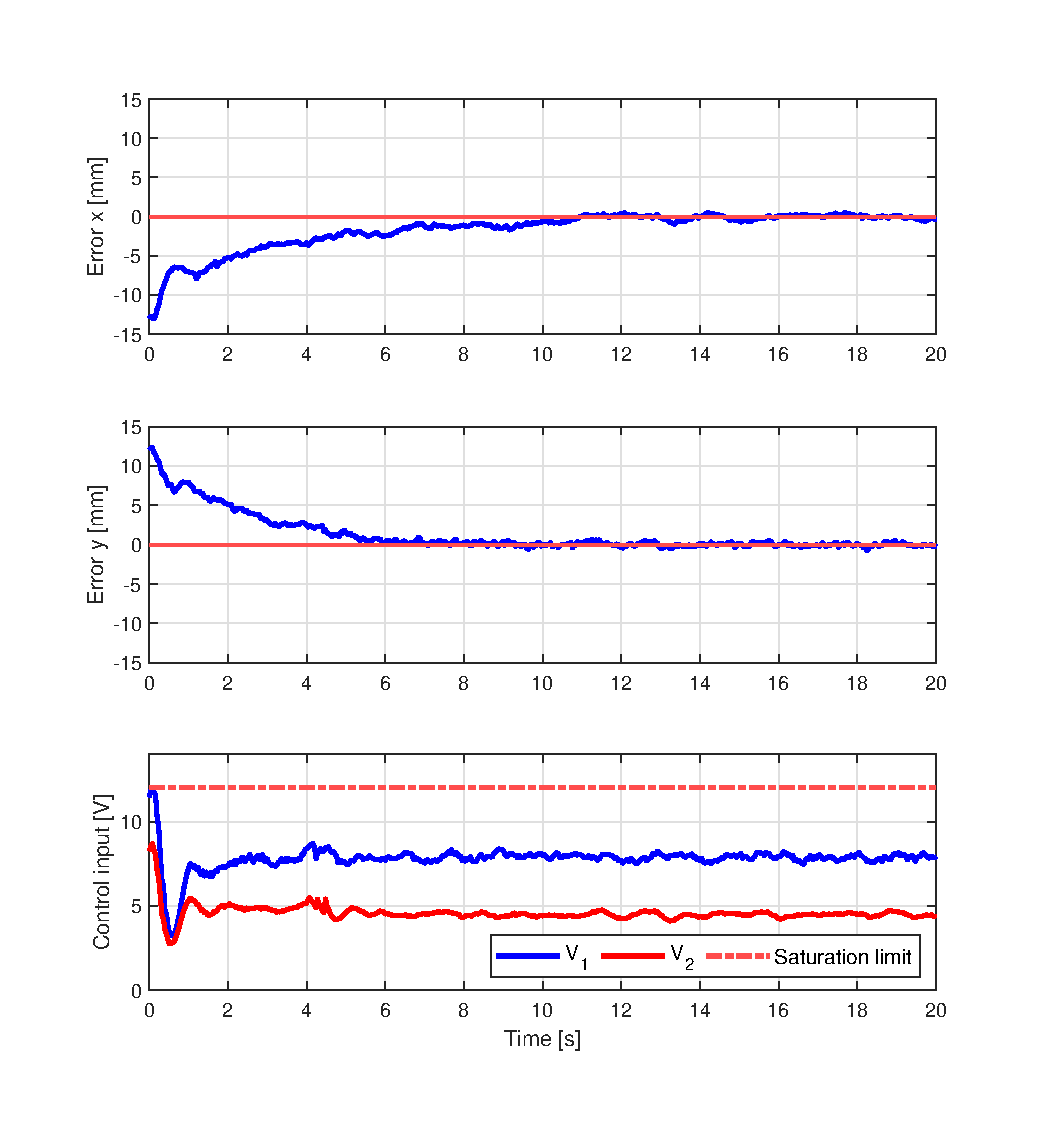
\includegraphics[width = 0.8\textwidth]{Figures/Chapter5/errorsignalleftwide.eps}
    \caption{\textbf{Top:} Error response of the x-coordinate. \textbf{Centre:} Error response of the y-coordinate. \textbf{Bottom:} Control input signal to the air-pumps.}
    \label{fig5:stepleft}
\end{figure}

\begin{figure}[H] 
    \begin{minipage}[b]{0.49\linewidth}
     \centering
    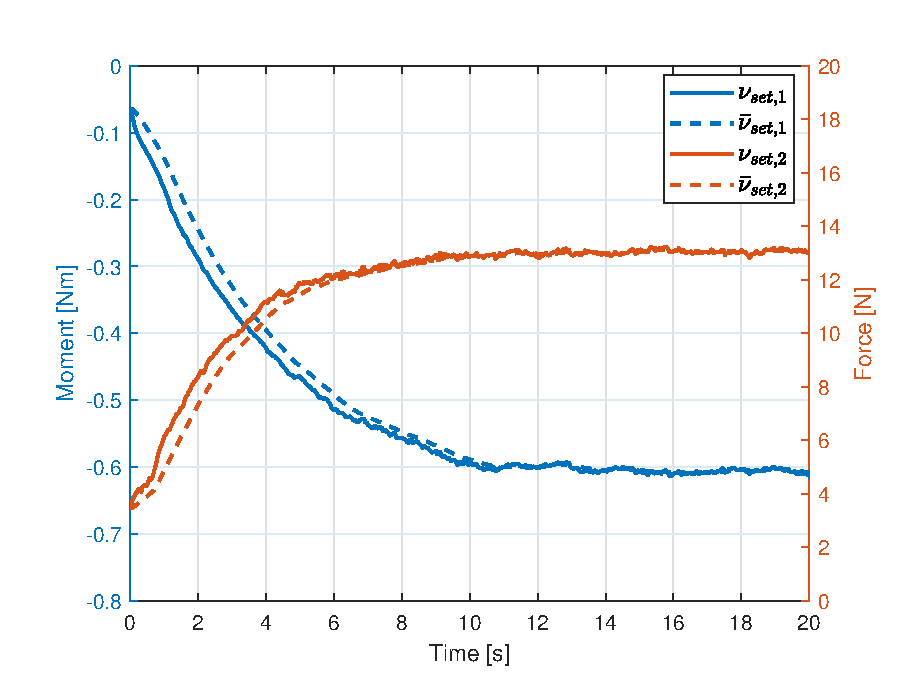
\includegraphics[width=\linewidth]{Figures/Chapter5/nuleft.eps} 
    \caption{Input moment and force as determined by Jacobian controller. Solid line is unfiltered input, dotted line low-pass filtered. } 
    \label{fig5:nuleft} 
       \end{minipage} 
    \begin{minipage}[b]{0.49\linewidth}
     \centering
    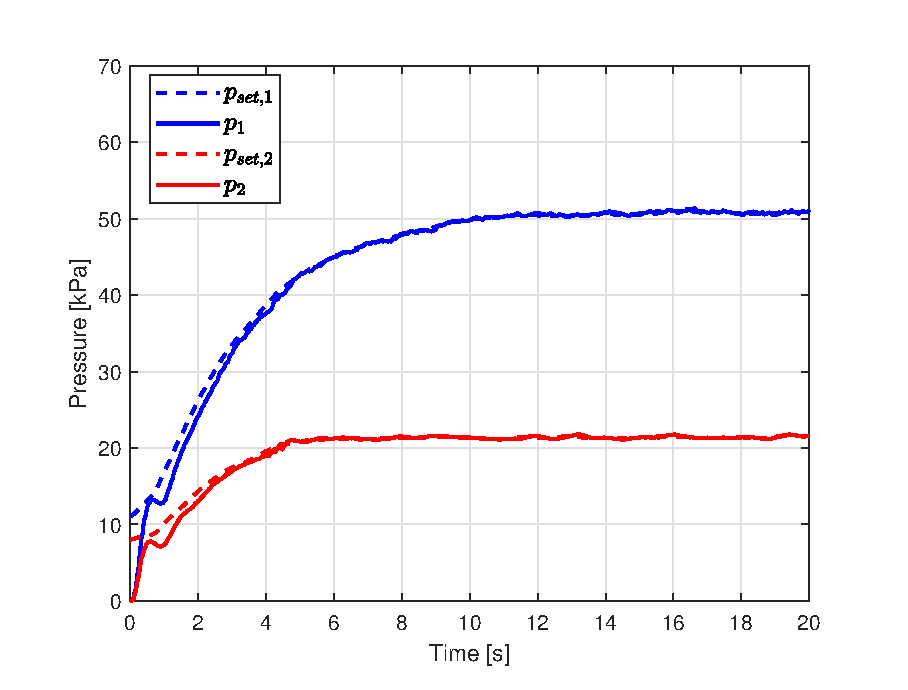
\includegraphics[width=\linewidth]{Figures/Chapter5/pressureleft.eps} 
    \caption{Pressure response, dotted lines indicate reference pressure, solid lines are measured pressures.} 
    \label{fig5:pleft} 
    \end{minipage} 
\end{figure}


As mentioned, the first set-point is mirrored to verify if the soft robot has equal characteristics when rotating in the opposite direction. The results of this setpoint, $r_{set} = [0.014,0.082]^\top$, are shown in Figure \ref{fig5:stepright}. This set-point is denoted as the ``right".


Again, the top plot shows the error in x-direction as a function of time. In comparison with the left set-point, this right set-point does not clearly show a swing during the first 2 seconds. Instead, a more gradual decrease in error is observed. After 13 seconds the zero error line is first crossed. From the input moment, as depicted in Figure \ref{fig5:nuright}, it can be seen that a steady-state is only reached after 20 seconds, at a value of $0.78 Nm$. Recalling, that a moment of $-0.6 Nm$ is necessary for the left set-point. Additionally, the bellow pressure $p_2$ reached a pressure of $60 kPa$ for the right setpoint, whilst for the left the set-point this was $51 kPa$. Based on these observations, it can be concluded that the curvature stiffness for positive rotation is larger than for negative rotation.

The error in y-direction for the right set-point shows equivalent behaviour as for the left set-point. The settling time is around 10 seconds which is 2 seconds more when compared to the first set-point. This can also be seen from force input in Figure \ref{fig5:nuright} which reaches a steady-state force of $15 N$.

The bottom figure of Figure \ref{fig5:stepright} shows the control volt send to the air pumps. The observed response is similar 
to the previous set-point. The oscillatory input during the first 1.5 seconds is caused by the proportional action. Then the integrator action becomes dominant over the proportional gain. Eventually the control input $V_1$ and $V_2$ stay close to 4.3 and 9.5 V, respectively. This voltage is higher compared to the left set-point, as the stiffness in this rotational directions seems to be higher. The control input to the motor also contains higher amplitude changes, which are linked to the noise on the pressure signal. Figure \ref{fig3:pump_dynamics_adapted} in Chapter \ref{chap3} showed that for higher pressures the noise floor increases. The noise effects can be observed in the controller input. To decrease these effects a low-pass filter on the pressure controller could be implemented, or the cut-off frequency of the low-pass filter on the pressure data could be decreased. However, both actions increase delays in the system which could cause stability problems.

Additional figures regarding the measured $x,y$ and $\theta$ position and modal coordinates can be found in Appendix \ref{app:chap5}.




\newpage
\begin{figure}[H]
    \centering
    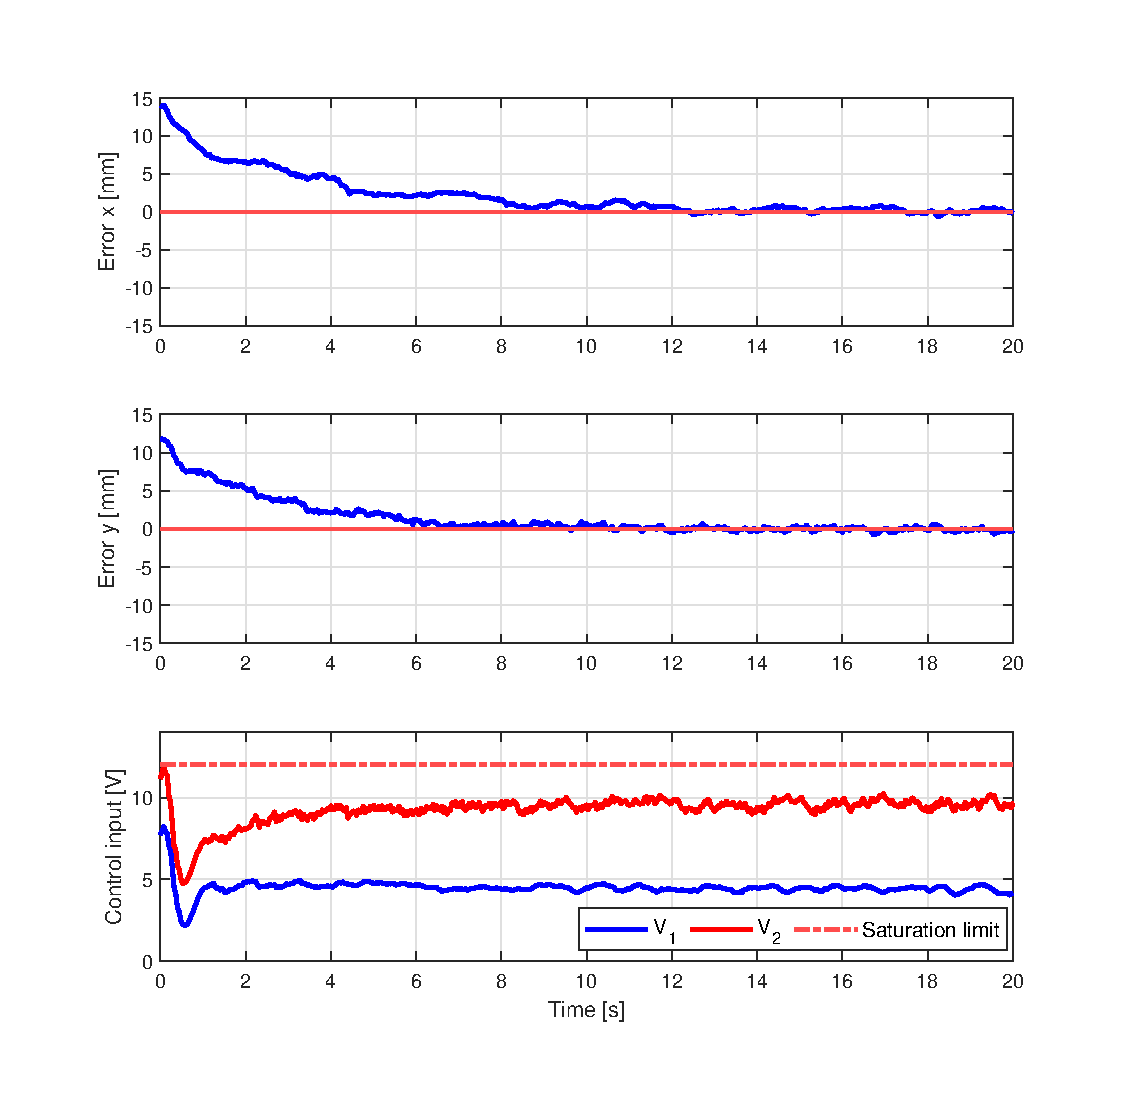
\includegraphics[width = 0.8\textwidth]{Figures/Chapter5/errorsignalright.eps}
    \caption{\textbf{Top:} Error response of the x-coordinate. \textbf{Centre:} Error response of the y-coordinate. \textbf{Bottom:} Control input signal to the air-pumps.}
    \label{fig5:stepright}
\end{figure}

\begin{figure}[H] 
    \begin{minipage}[b]{0.49\linewidth}
     \centering
    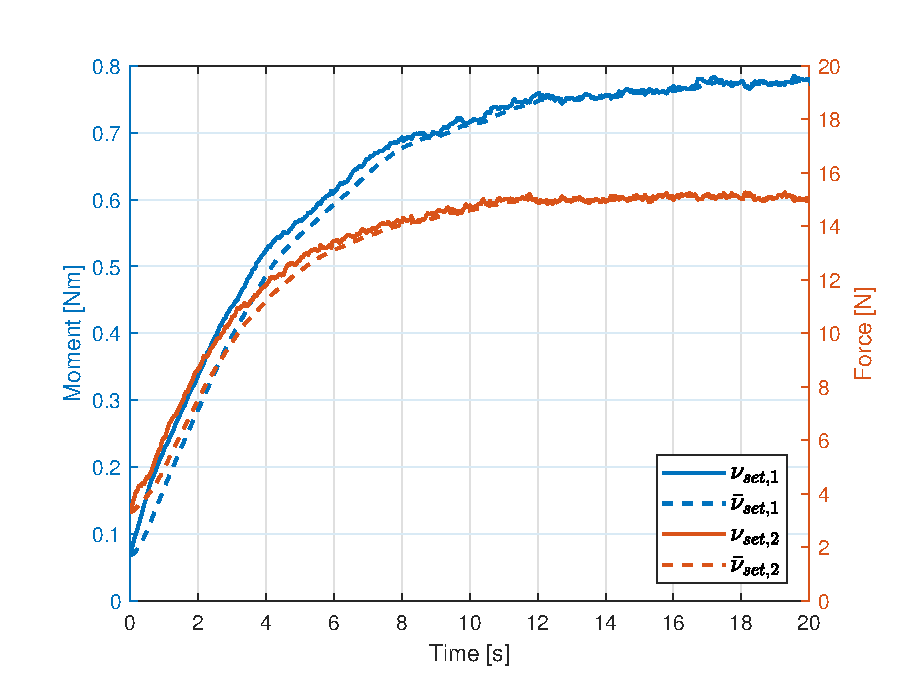
\includegraphics[width=\linewidth]{Figures/Chapter5/nuright.eps} 
    \caption{Input moment and force as determined by Jacobian controller. Solid line is unfiltered input, dotted line low-pass filtered. } 
    \label{fig5:nuright} 
       \end{minipage} 
    \begin{minipage}[b]{0.49\linewidth}
     \centering
    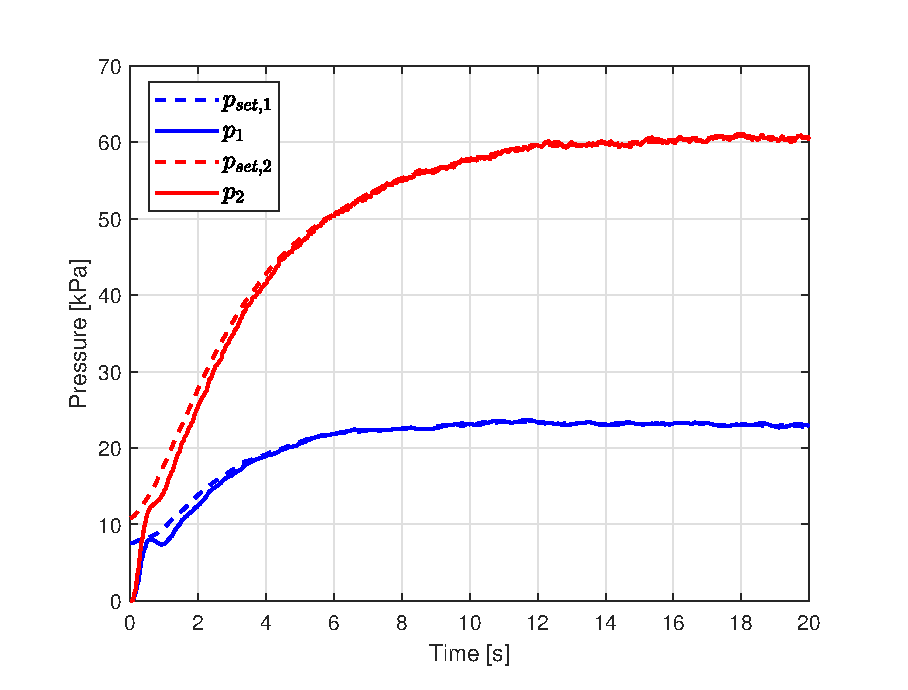
\includegraphics[width=\linewidth]{Figures/Chapter5/pressureright.eps} 
    \caption{Pressure response, dotted lines indicate reference pressure, solid lines are measured pressures.} 
    \label{fig5:pright} 
    \end{minipage} 
\end{figure}



For both set-points the Root-Means-Square (RMS) error is analysed after the control input $\nu$ reaches its steady-state control input. To this end, an experiment for more than 20 seconds is carried out. The obtained error values are presented in Table \ref{tab:RMSerrors}. It can be seen that the RMS error for the right set-point is larger compared to the left set-point. The cause of this problem is related to the stiffness properties of the actuator. The curvature stiffness for positive and negative rotation is not uniform. This could be related to manufacturing tolerances, e.g. the material thickness of both bellows is not equal. Other possibilities can relate to the elastomer itself, e.g. exposure time of the laser or the time interval between each printed layer. 



\begin{table}[H]
    \centering
    \caption{RMS error after 15 seconds}
    \begin{tabular}{|c|c|c|} \hline
     Set point $[x,y]^\top$    & $e_{RMS,x}$ $mm^2$  &  $e_{RMS,y}$ $mm^2$  \\ \hline
    Left $r_{set}= [-0.014,0.082]^\top$     & 2.6034e-04  & 2.2644e-04 \\ \hline
    Right $r_{set}= [0.014,0.082]^\top$  &  3.2692e-04 &   2.6577e-04\\ \hline
    \end{tabular}
    \label{tab:RMSerrors}
\end{table}




\section{Reference tracking in experiments}

To evaluate the performance of the controller during a reference tracking problem we analyze the tracking of an ellipsoid reference signal. The equations describing this ellipsoid as function of time are given as,

\begin{equation}
    x_{ref} = \begin{cases} 
      0 &  t \leq t_1 \\
     \alpha \sin(2\pi \frac{t - t_1}{T_{ell}}) & t \leq T_{ell} + t_1 \\
     0 & t > T_{ell} + t_1
   \end{cases} 
\end{equation}

and,


\begin{equation}
    y_{ref} = \begin{cases} 
      \frac{(y_{off} - L) t}{t_1} &  t \leq t_1 \\
     (y_{off} +\beta) -  \beta \cos(2\pi \frac{t - t_1}{T_{ell}}) & t \leq T_{ell} + t_1 \\
     y_{off} & t > T_{ell} + t_1
   \end{cases} 
\end{equation}


where it can be seen that during the first $t_1$ seconds the reference position linearly increases to an offset $y_{off}$. Then, clockwise rotation occurs during $T_{ell}$ seconds in which the amplitude in the x-direction is $\alpha$, and the maximum elongation in y-direction is $y_{off} + \beta$. Once the ellipsoid has been completed, the reference signal is equal to its offset position. The values of these parameters are shown in Table \ref{tab5:refparams}. Since the controller has no feedforward control, and settling times are at least 15 seconds in the x-direction, $T_{ell}$ is chosen 60 seconds. The amplitudes, $\alpha$ and $\beta$ are comparable to the set-points presented in the previous section. 


\begin{table}[H]
    \centering
    \caption{Reference tracking parameters}
    \begin{tabular}{|c|c|} \hline
   \textbf{Paramter}  & \textbf{Value [unit]} \\ \hline
    $t_1$ &   10 [s]  \\ 
    $\alpha$ & 13 [mm] \\
    $\beta$ & 7 [mm] \\
    $T_{ell}$ & 60 [s] \\ \hline
\end{tabular}
    \label{tab5:refparams}
\end{table}

The results of the above reference trajectory a plotted in Figure \ref{fig5:errorellips}. The left-hand figure shows the position in the x,y plane as a solid blue line, whereas the reference is plotted as a dotted black line. Additionally, green crosses mark the reference position at a given time, whereas red crosses mark the actual position at a given time. It can be seen that the actual position is lagging behind the reference position. This phenomenon is caused by the low-pass filter of the model-based controller, preventing rapid changes in the reference moments and force. This problem can be resolved by increasing $T_{ell}$. Therefore the error response as shown on the right-hand side of Figure \ref{fig5:errorellips} is not an accurate representation of the soft robot's capabilities.

Another observation is the high-frequency noise in the position measurement. The origin of this noise is caused by the air pumps. 
The bottom figure in Figure \ref{fig5:controlellips}, shows the control input to the air-pumps. This figure shows that especially in regions where the volt input approaches saturation levels large-amplitude volt changes occur. This coincides with the pressure step response as presented in Chapter \ref{chap3}, which showed increasing noise levels for pressure increases. Although the pressure data is low-pass filtered, spikes in the volt control input still occur. 

Furthermore, the effect on non-symmetrical material properties can be observed in Figure \ref{fig5:errorellips}. Tracking the reference in the positive x domain seems to cause higher errors, compared to the negative x domain. Especially between 20 and 30 seconds, the actual position deviates much from the reference set-point. For a large part, the set-point is not even reached at all. In the negative x-domain, between 50 and 60 seconds, relative large position errors are observed as well. However, the position error in this region contains both positive and negative errors, indicating that the set-point is reachable. Since the task-space has not been determined it remains hard to tell if the entire ellipsoid is situated in the robots task-space. 
\newpage

\begin{figure}[H]
    \centering
    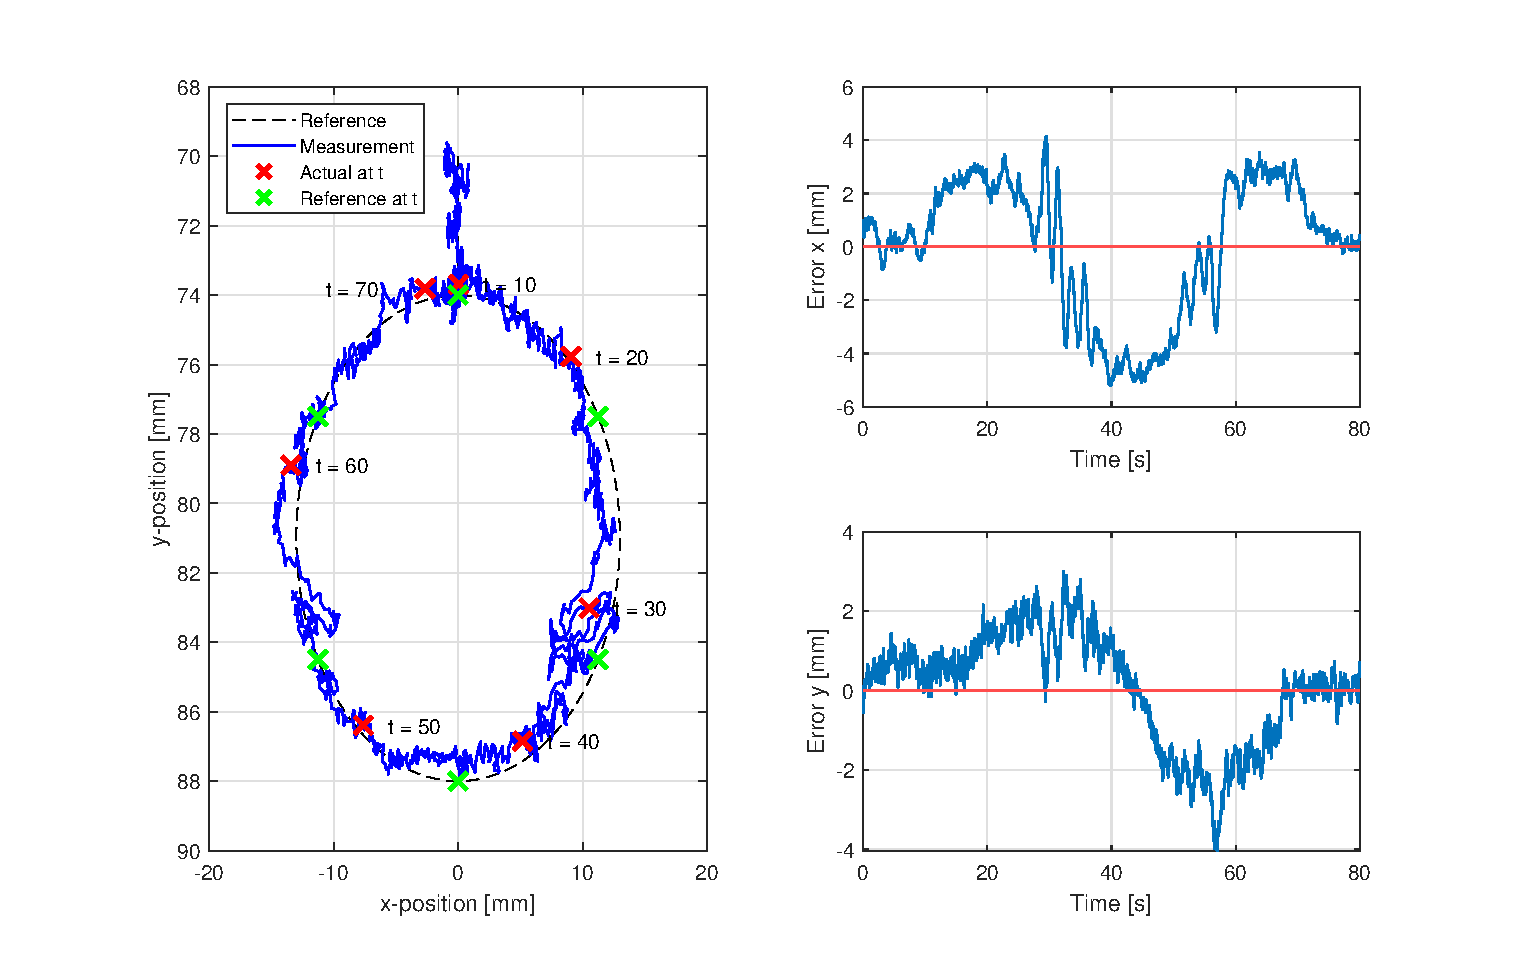
\includegraphics[width = \textwidth]{Figures/Chapter5/error.eps}
    \caption{\textbf{Left:} Position of the end-effector in the x,y plane with time stamps. \textbf{Right top:} Error signal as a function of time in x-direction. \textbf{Right bottom:} Error signal as a function of time in y-direction.}
    \label{fig5:errorellips}
\end{figure}


\begin{figure}[H]
    \centering
    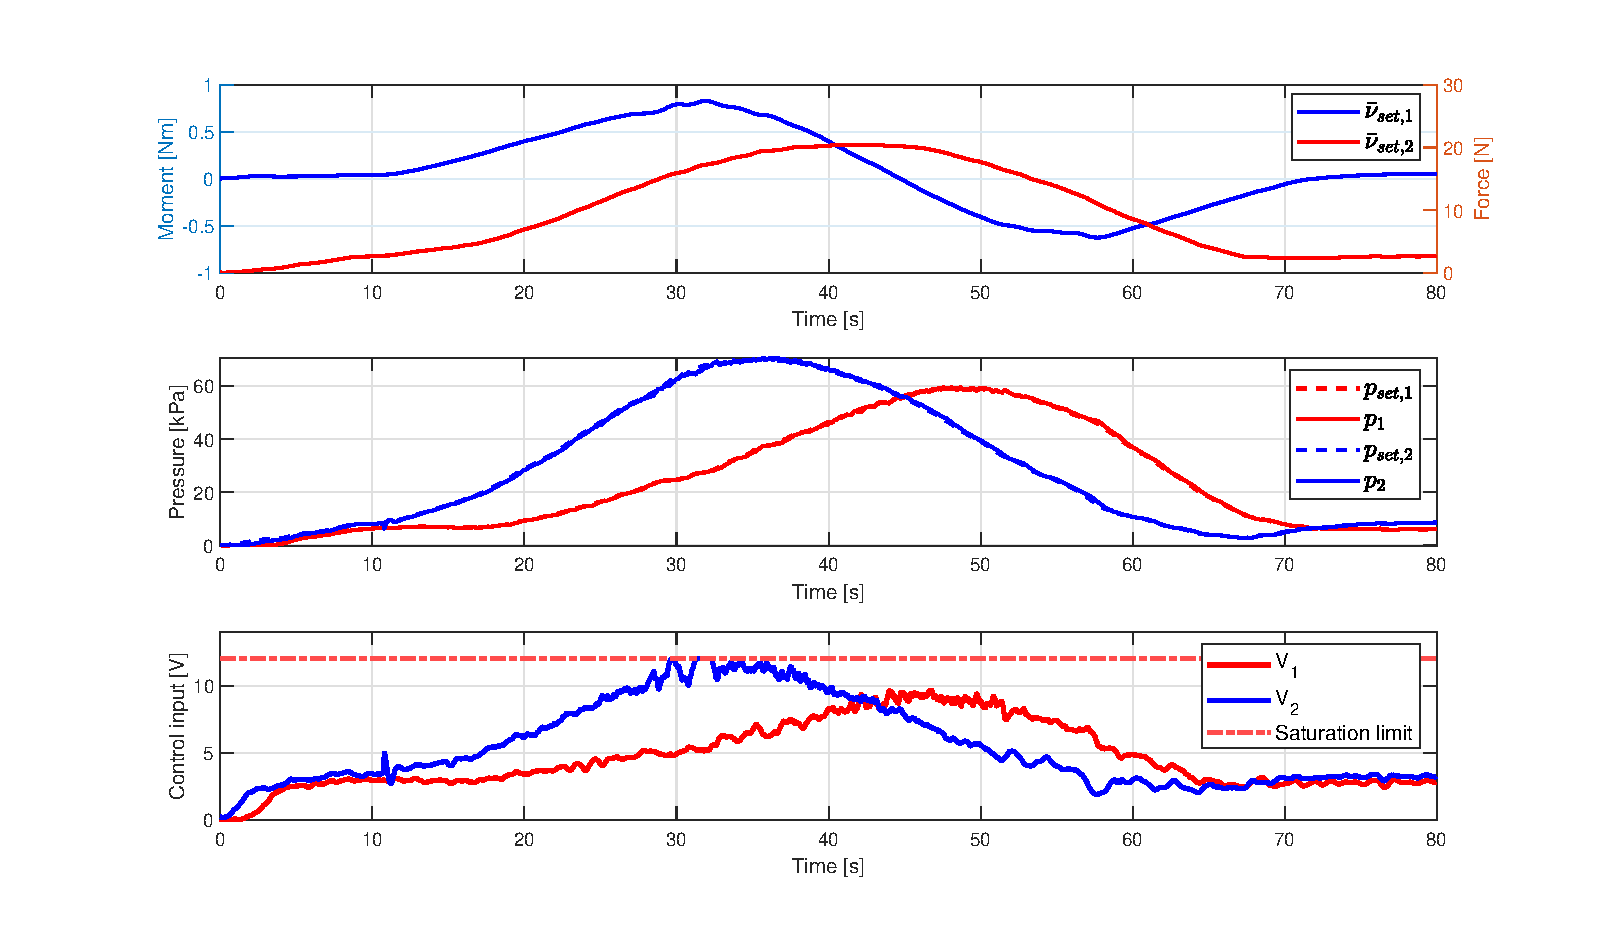
\includegraphics[width = \textwidth]{Figures/Chapter5/controlsignalextend.eps}
    \caption{\textbf{Top:} Control signal of model-based controller. \textbf{Middle:} Reference pressure and measured pressure. \textbf{Bottom:} Control input to the air-pumps.}
    \label{fig5:controlellips}
\end{figure}

The unsymmetrical material properties are visualized by a pressure contour plot, as depicted in Figure \ref{fig5:pressureellips}. In this figure, the red crosses indicate time stamps. The solid black line indicates the pressures at which the actuator should theoretically only elongate. Perpendicular to this black line, red lines mark elongation and curvature set-points. Previously, it was assumed that the soft robot deforms symmetrically during rotation. However, this statement holds up til a pressure of about 50 kPa. The red lines $a_1$ and $a_2$ are of equal lengths and are close to measured pressures. This also holds for the lines $b_1$ and $b_2$. Considering pressures above 50 kPa, the symmetry argument does not hold. The lines $c_1$ and $c_2$ are not of equal length, indicating that curvature stiffness is dependent on its sign. 




\begin{figure}[H]
    \centering
    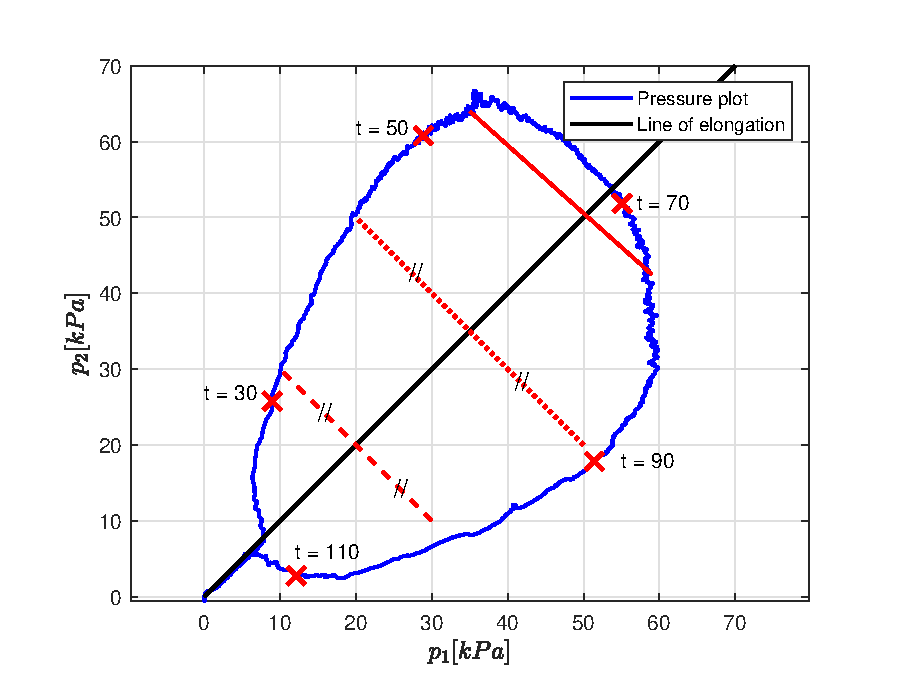
\includegraphics[width = 0.8\textwidth]{Figures/Chapter5/pressurecontour.eps}
    \caption{Contour plot of the bellow pressure $p_1$ and $p_2$, red lines indicate (non)-symmetrical material properties.}
    \label{fig5:pressureellips}
\end{figure}








% Sample frequency arduino = 25 millisecond is 40 Hz Sample frequency Raspberry pixymon onn= 58 millisecond = 18.5HzSample freq Raspberyy pixymon off = 40 millisecondsPixymon off max sample freq = 40Hz, 25 millisecondpixymon on max sample freq = 20 Hz, 50 millisecond



%The effects of clockwise rotation also effect the observed response. The deflation rate is dependent on the porousness of the soft robot and actual pressure. Therefore, decreasing volt input does not result in instant pressure decrease. Therefore, $T_{ell}$ must be . 



%in high voltage regions  Between 27 and 38 seconds the volt input to the air pumps approaches saturation levels. At this exact time, major spikes occur in the error response in both x and y-direction.



%First, the low-pass filter on the model-based controller , as seen in the top figure. Therefore, the controller is not able to respond to relatively quick changes in the reference signal. The second reason can be explained by the pump dynamics. These air-pumps act as a first-order system, with comparable behaviour of a low-pass filter. This means that when increasing the input voltage, pressure changes are not observed instantly. In Figure \ref{fig}




%It immediately becomes clear that a time progresses, the tracking error between reference and actual position increases. \textbf{TODO}. Although this lagging is observed, the soft robot is still able to track the reference position relatively well, given the delay. The error plots in x and y direction are plot on the right hand side of Figure \ref{fig5:errorellips}. These plots do not well represent the tracking capabilities of the controller, as the reference signal is too fast to track. Consider Figure \ref{fig5:controlellips}  It can be seen that the control input as determined by the model based controller only shows some oscillation around 31 and 58 seconds. This times coincide with the . Only small For the input of the model-based controller and pressure response noise levels are low. However, it can be seen that based on. 



%\textbf{todo, redo this experiment. increase Tell and do a clockwise and counter  clockwise experiment. As deflation can not actively be done}
